\subsection*{Novos Gráficos}
\begin{tcolorbox}
Dada uma função $f:X\longrightarrow \mathbb{R}$, podemos obter novos gráficos fazendo uma translação do gráfico de $f$ ao longo do eixo $x$ ou ao longo do eixo $y$.

\subsubsection*{Translações de Gráficos de Funções}

\begin{figure}[H]
\centering
\subfigure{
    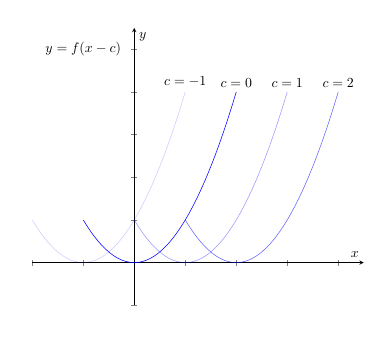
\begin{tikzpicture}[scale=0.5]
\begin{axis}[
 axis lines=middle,
 ticklabel style={fill=white},
xmax=4.5,
 ymin=-1,ymax=5.5,
 xlabel=$x$,ylabel=$y$,
 samples=100,
 smooth,
% xtick={-1,0,1.5}, ytick={-1,1},
xticklabels=\empty, yticklabels=\empty,
 width=10cm]
% \coordinate  (x2) at (1,1);
% \coordinate  (x1) at (-1,-1);
\addplot[blue,  domain=-2:1, opacity=0.2] {(x+1)^2};
\addplot[blue,  domain=-1:2] {x^2};
\addplot[blue, domain=0:3, opacity=0.4] {(x-1)^2};
\addplot[blue, domain=1:4, opacity=0.6] {(x-2)^2};
%\addplot[blue] {(x-2)^2};

% \draw[dashed] (-1.5,0) --(-1.5,{0.5*sin(deg(-1.5)}) --(0,{0.5*sin(deg(-1.5)}) ;

% \draw[dashed] (1.5,0)  -- (1.5,{0.5*sin(deg(1.5)})--(0, {0.5*sin(deg(1.5)});
\node[] at (axis cs:-1,5) {$y=f(x-c)$};

% \node[right] at (axis cs:0, {0.5*sin(deg(-1.5))}) {$-f(a)$};
% \node[left] at (axis cs:0, {0.5*sin(deg(1.5))}) {$f(a)$};
\node[above] at (axis cs:1, 2^2) {$c=-1$};
\node[above] at (axis cs:2, 2^2) {$c=0$};
\node[above] at (axis cs:3, 2^2) {$c=1$};
\node[above] at (axis cs:4, 2^2) {$c=2$};
\end{axis}
\end{tikzpicture}}
    \qquad
\subfigure{
    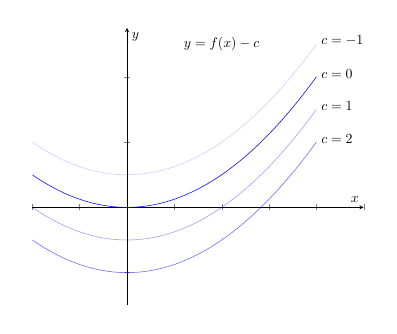
\begin{tikzpicture}[scale=0.5]
\begin{axis}[
 axis lines=middle,
 ticklabel style={fill=white},
xmax=2.5,
 ymin=-3,  ymax=5.5,
 xlabel=$x$,ylabel=$y$,
 samples=100,
 smooth,
xticklabels=\empty, yticklabels=\empty,
 width=10cm]

\addplot[blue,  domain=-1:2, opacity=0.2] {(x)^2+1};
\addplot[blue,  domain=-1:2] {x^2};
\addplot[blue, domain=-1:2, opacity=0.4] {(x)^2-1};
\addplot[blue, domain=-1:2, opacity=0.6] {(x)^2-2};
%\addplot[blue] {(x-2)^2};
\node[] at (axis cs:1,5) {$y=f(x)-c$};
\node[right] at (axis cs:2,2^2+0.1) {$c=0$};
\node[right] at (axis cs:2,2^2+1+0.1) {$c=-1$};
\node[right] at (axis cs:2,2^2-1+0.1) {$c=1$};
\node[right] at (axis cs:2,2^2-2+0.1) {$c=2$};
\end{axis}
\end{tikzpicture}}
\end{figure}
\end{tcolorbox}
